\documentclass[11pt]{article}
\usepackage{graphicx}
\usepackage{amssymb}
\usepackage{epstopdf}
\DeclareGraphicsRule{.tif}{png}{.png}{`convert #1 `basename #1 .tif`.png}

\textwidth = 6.5 in
\textheight = 6.5 in
\oddsidemargin = 0.0 in
\evensidemargin = 0.0 in
\topmargin = 0.0 in
\headheight = 0.0 in
\headsep = 0.0 in
\parskip = 0.2in
\parindent = 0.0in

\newtheorem{theorem}{Theorem}
\newtheorem{corollary}[theorem]{Corollary}
\newtheorem{definition}{Definition}

\title{Examples of Scientific Computing via Wavelets}
\author{Daniel Beatty}
\begin{document}
\maketitle

\newpage
\section {Methods of Computing Wavelets}
\subsection{Convolution}
Typically, each component has the form $O\rightarrow (A|D)$ where 
\begin{itemize}
\item  O is the original signal
\item A is the average component
\item D is the difference component 
\item $(A|D)$ the signal A concatenated with D. 
\end{itemize}

The general algorithm is 

$\forall i\in \lbrack 0,M)$

\qquad $\forall j\in \lbrack 0,N)$

\qquad \qquad n=i-j

\qquad \qquad if ($n\in \lbrack 0,M)$)

\qquad \qquad \qquad $y_{i\,}+=x_{n}\cdot h_{j\,}$

1-D Convolution is fairly straight forward from the algorithm.  

 
\subsection{2-D Convolution}
2-D Convolution is little more complicated, and requires a choice in the manner in which it is computed.  For speed, the choice is perform the operation directly on each row and then each column of the matrix.  

$\forall i  \in rows in the matrix$
\begin{itemize}
\item Generate $S \stackrel{\phi}{\to} A$ on row i
\item Generate $S \stackrel{\psi}{\to} D$ on row i
\item Unite $A concat D \to (A|D) $ in row i of $W^\prime $
\end{itemize}

$\forall j  \in columns in the matrix$
\begin{itemize}
\item Generate $W^\prime \stackrel{\phi}{\to} A$ on column j
\item Generate $W^\prime \stackrel{\psi}{\to} D$ on column j
\item Unite $A concat D \to (A|D) $ in column j of $W^\prime $
\end{itemize}

\newpage
\subsubsection {Chosen Method}
The algorithm is as follows for the row tranform (and is similar for the column transform):  

$\forall i \in rows$
\begin{enumerate}
\item Initialize temporary array/vector to all zeros (x).
\item $\forall k \in columns $
\begin{enumerate}
\item $\forall l \in ha.Size $
x +=  \begin{tabular}{ll}
$S_{i,k-l} * hA_l$ & $k-l \in columns$ \\ 
$0$ & $otherwise$%
\end{tabular}
\end{enumerate}
\item $\forall k \in columns/2 $

$result_{i,k} = x_{2k+1} $  (In other words, odd split)

\item Initialize x to all zeros.
\item $\forall k \in columns $
\begin{enumerate}
\item $\forall l \in hd.Size $
x +=  \begin{tabular}{ll}
$S_{i,k-l} * hD_l$ & $k-l \in columns$ \\ 
$0$ & $otherwise$%
\end{tabular}
\end{enumerate}

\newpage
\subsection{1-D Storage Method}
The obvious choice is to take either the odd or even indexed values of the average and difference over complete forms, and insert them into the array such that all of the averages are followed by the difference.  Each component is subsequently a complete wavelet packet.  

\subsection{2-D Storage Method}
The matrix form below is chosen for its simplicity:

$\qquad B\Rightarrow 
\begin{tabular}{ll}
$A$ & $V$ \\ 
$H$ & $D$%
\end{tabular}
$

begin{enumerate}
\item Average component: produced by filtering the row vectors and the column vectors with the averaging filter.
\item Vertical Component:  produced by applying the average filter to the column vectors and the difference filter to the row vectors.
\item Horizontal component: produced by applying the average filter to the row vectors and the difference to the column vectors.
\item Diagonal component: produced by applying the difference filter to both the row and column vectors.  
\end{enumerate}

\newpage
\subsection {Multi-Resolution}

The wavelet transform (multiresolution) uses private members of the class (hA, hD, xD/yD, xA/yA).  Both Haar filters are maintained this way.  Also both row and column transforms have average and difference myVector classes for temporary storage.   All of these members are allocated and destroyed by the wavelet transform method itself.   The simplified algorithm of the row transform is the following:
\begin{enumerate}
\item Initialize xA and xD to zero
\item $\forall k \in columns \forall l \in filter$
\begin{itemize}
\item n = k - l
\item if ( $n \in columns $ )

	$xA_k = W_{i,n} * hA_l $
	
	$xD_k = W_{i,n} * hD_l $
	
	
\end{itemize}
\item Transfer back to W

	$W_i = xA|xD $
\end{enumerate}

\begin{enumerate}
\item initialize yA and yD to zero
\item $\forall k \in rows \forall l \in filter$
\begin{itemize}
\item n = k - l
\item if ( $n \in columns $ )

	$yA_k = W_{i,n} * hA_l $
	
	$yD_k = W_{i,n} * hD_l $
	
	
\end{itemize}
\item Transfer back to W

	$W_j = yA|yD $
\end{enumerate}

\section{Computation Costs}
\subsection {For 1-D operations}
Linear Cost
\subsection {2-D Operations}
Cost is inherently $O(N^2)$

\newpage
\section {Results}
\subsection { 1-D Transform}
Testing of the 1-D wavelet was performed on a sinusoidal wave form of 128 elements.  The given function has the equation shown in Figure \ref{sample}.

$y[n] = 10 \sin (\frac{n}{128}) - 5 \sin (\frac{n}{64}) + 2 \sin (\frac{3n}{128}) - \sin (\frac{n}{32})$

Also this produces a functional difference between wavelet inverse transform for odd and even versions.  The difference is slight; however, the last element is lost in the even indexed form.  

\begin{itemize}
\item Odd   $R_{2i} =(A_i - D_i ) \sqrt{1/2} $
	$R_{2i+1}=(A_i + D_i ) \sqrt{1/2} $
\item Even $R_{2i} =(A_i + D_i ) \sqrt{1/2} $
	$R_{2i-1}=(A_i - D_i ) \sqrt{1/2} $
\end{itemize}
\newpage

\begin{figure}
\includegraphics [width=4in]{sample.jpg}
\caption{Sample function.  The x-axis is the array index (index n).  The y value is simple -- the value y[n]. }
\label{sample}
\end{figure}



\begin{figure}
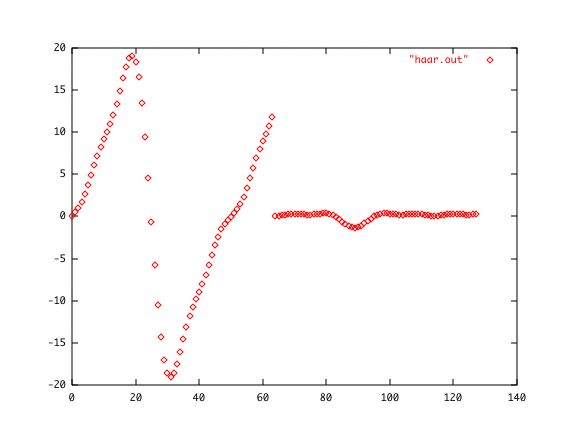
\includegraphics [width=4in]{recovered.jpg}
\caption{Recovered function.  The x-axis is the array index (index n).  The y value is simply the value y[n].  The function was recovered from an odd indexed wavelet transform. }
\label{recoverOdd}
\end{figure}

\begin{figure}
\includegraphics [width=4in]{sample.jpg}
\caption{Recovered function.  The x-axis is the array index (index n).  The y value is simply the value y[n].  The function was recovered from an even indexed wavelet transform. }
\label{recoverEven}
\end{figure}


\subsection { 2-D Pictures}


\begin{figure}
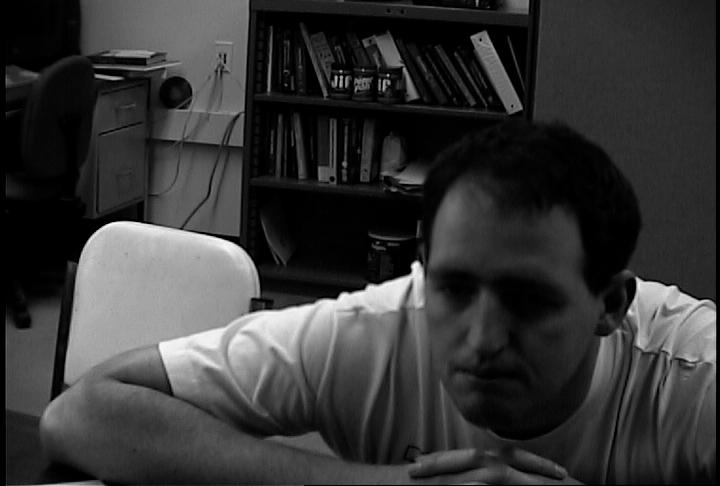
\includegraphics [width=4in]{rightDan.jpg}
\caption{Original Image.  This image is the original image. }
\label{rightDan}
\end{figure}

\begin{figure}
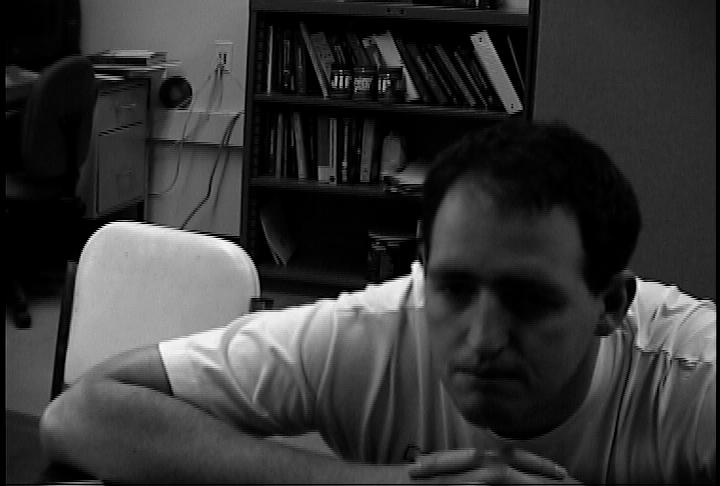
\includegraphics [width=4in]{revRecover.jpg}
\caption{Recovered Image.  This image is the recovered image.  Depending on whether the image was saved as a picture first can affect the white spots in the picture.  Ringing is also an issue.  }
\label{rightDanRecovered}
\end{figure}

\begin{figure}
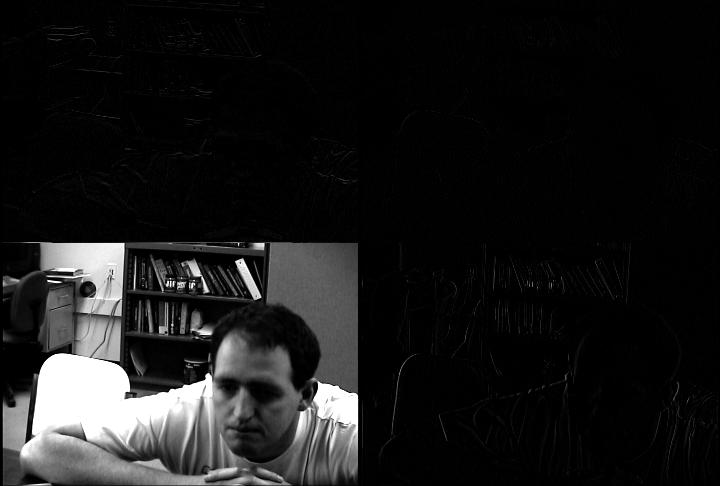
\includegraphics [width=4in]{revWavepic.jpg}
\caption{Wavelet Transform Image.  This image is divided in to average, horizontal, vertical and diagonal components. }
\label{rightWavepic}
\end{figure}


\begin{figure}
\includegraphics [width=4in]{selfWavepic.jpg}
\caption{Wavelet Transform Image.  This image is divided in to average, horizontal, vertical and diagonal components, using the vector-matrix version. }
\label{wavepic}
\end{figure}

\begin{figure}
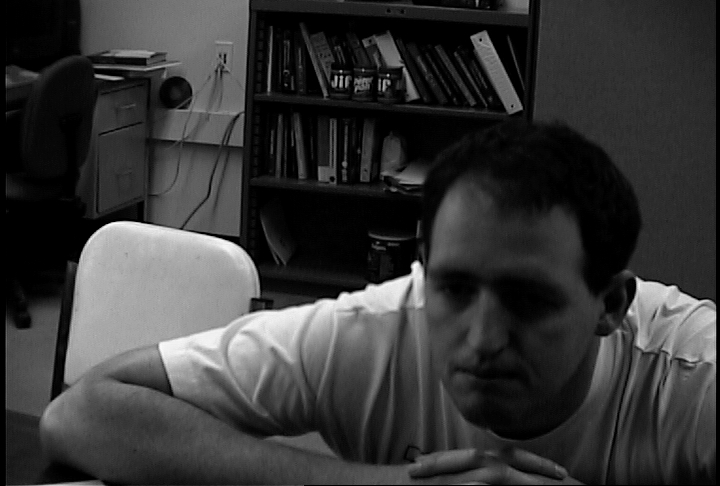
\includegraphics [width=4in]{selfRecover.jpg}
\caption{Recovered Image (Vector-Matrix Method).  This image is the recovered image.  This version avoids the ringing by using the vector-matrix version which is more aligned for the inverse wavelet transform.  }
\label{rightDanRecovered}
\end{figure}

\begin{figure}
\includegraphics [width=4in]{wavepic3R.jpg}
\caption{Wavelet Transform Image.  This image is divided in to average, horizontal, vertical and diagonal components using multi-resolution wavelet transform.  Note the the average component was transformed one step further. }
\label{wavepicR3}
\end{figure}

\newpage
More Pictures
\newpage
More pictures
\newpage

\section{Matrix Multiplication}
\subsection{Simple Proof}
A reminder from Dr. Sinzinger, wavelets and their inverses are linear operators.  As he correctly reminded me any linear operator has the following properties:

\begin{enumerate}
\item $L(AB) = L(A) \dot L(B)$
\item $\psi ^{-1}$ is a linear operator
\item $\psi ^{-1} (\psi (A) \dot \psi (B)) = \psi ^ {-1} (\psi (A)) \dot \psi ^{-1} (\psi(B)) $
\item $\psi ^{-1}(\psi(A)) = A$
\item $\psi ^{-1}(\psi(B)) = B$
\item Therefore:  $AB = \psi^{-1} (\psi(A) \dot \psi(B))$  
\end{enumerate}

Thus this is sufficient proof that wavelet matrix multiplication is sound.  

\subsection { Limits spelled out by the proof}
One catch-22 to be had with the simple proof.  The linear transform has to be the same linear transform on both matrices.  If the matrices are the same size, ($N\times N$) then this is no-brainer.  If they are $M \times P$ and $P\times N$, then it is not clear that the wavelet transforms of each are the same operator.  

\newpage
\subsection {Chain Link Structure}
Class Chain Link 
members:
length 
hooks

Class Hook 
members:
length
l2norm
links 

Class Link
members: 
id
value

\newpage

\section {Items to come}
\subsection {Matrix Inversion}
\subsection {PDE's in Wavelet Space}

 \end{document}